\chapter{Background and Related Works}\label{ch:background}

\section{Neural network architecture}\label{sec:nn-architecture}

Broadly speaking, a neural network can be described as a certain layering of nodes, or \textit{units}, connected to each other by directed \textit{links}, where each link has a certain numeric weight that signifies the strength of connection between the connected nodes. 

Historically, the concept of `net of neurons' whose interrelationship could be expressed in propositional logic was first proposed by~\cite{McDPit43} in 1943, inspired by a ``all-or-none" behaviour of the biological nervous system. The first basic unit, also called the \textit{perceptron}, was invented by~\cite{Ros62}. A perceptron will be activated if the sum of all the input values from its input links, say $x_1,..., x_m$, multiplied by the links' corresponding weights, say $\theta_1,..., \theta_m$, is above that unit's certain threshold value, or \textit{bias} $b$, such that
\[ \text{output} = 
   \begin{cases}
   0 & \quad \text{if } \displaystyle\sum_{i=1}^{m} x_i \theta_i \leq b\\
   1 & \quad \text{otherwise }
   \end{cases}
\]

The above is equivalent to vectorizing the inputs to $\boldsymbol{x} = [x_1,...,x_m]$, weights to $\boldsymbol{\theta} = [\theta_1,...,\theta_m]$ and inverting the sign on $b$, so that,
\[ \text{output} = 
   \begin{cases}
     0	& \quad \text{if } \boldsymbol{x} \cdot \boldsymbol{\theta} + b \leq 0\\
     1	& \quad \text{otherwise }
   \end{cases}
\]

\begin{figure}
  \centerline{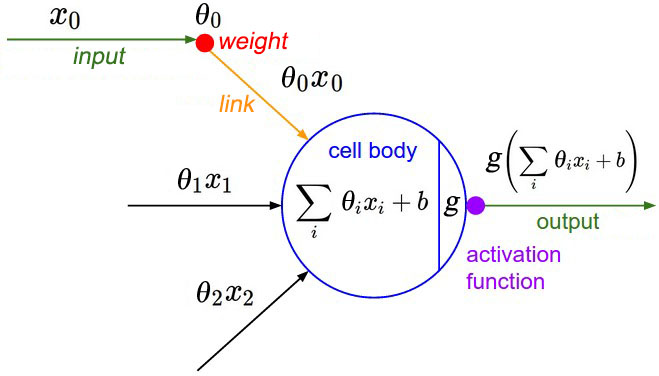
\includegraphics[width=0.7\linewidth]{neuron_model.jpg}}
  \caption{Structure of a modern unit by~\cite{Kar16}.}
  \label{fig:neuron}
\end{figure}

The perceptron eventually evolved into the modern unit, which computes the output value as a \textit{range} of values, obtained by applying an \textit{activation function} to the sum of its inputs and bias. With this modification, a small change in the inputs only resulted a small change in the output, allowing a more convenient way to gradually modify the weights and consequently, improve the learning algorithm~\cite{Nie16}.

There are various activation functions; historically, the most commonly used is the \textit{sigmoid} function, $\sigma(x) = 1/(1+e^{-x})$. Its advantages and disadvantages are outlined in \ref{se:previmplem}.~\cite{Kar16} recommends using less expensive functions with better performance, such as,
\begin{enumerate}
\item Tanh function, $tanh(x) = 2\sigma(2x)-1$.
\item Rectified Linear Unit (ReLU) function, $f(x)=max(0,x)$.
\item Leaky ReLU function, $f(x) = 1(x < 0)(\alpha x) + 1(x >= 0)(x)$
\item Maxout function, $max(w_{1}^{T}x + b_{1}, w_{2}^{T}x+b_{2})$.
\end{enumerate}

\begin{figure}
  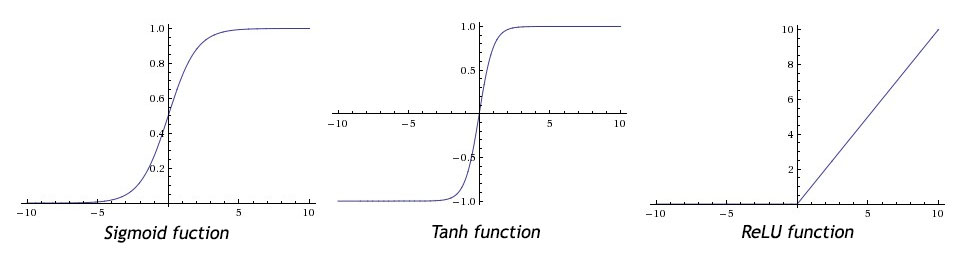
\includegraphics[width=\linewidth]{activation-functions.jpg}
  \caption{Graphs of some common activation functions~\cite{Kar16}.}
  \label{fig:activation-graphs}
\end{figure}

A unit's output can be expressed as $g(\boldsymbol{x} \cdot \boldsymbol{\theta} + b)$, where $g(x)$ is the chosen activation function.

As previously mentioned, the general architecture of a neural network can be described as distinct layers of these units, which are connected to units in its adjacent layers. The most common layer type is \textit{fully-connected}, which means that each unit in a layer is connected to every unit in the adjacent layer~\cite{Nor14}. 

The \textit{input layer} receives input values corresponding to the number of features\footnote{For instance, in a $200 \times 200$ pixel image recognition problem, there may be $40,000$ features corresponding to each individual pixel's RGB values.} in the neural network. The last, or \textit{output layer} usually corresponds to different classes in a multi-classification problem, or some real-valued target in a regression problem~\cite{Kar16}. The layers in between input and output layers are called \textit{hidden layers}; a neural network is classified as DNN if it contains more than one hidden layer. Increasing the size and numbers of hidden layers also increases the \textit{capacity} of the neural network~\cite{Kar16}; that is, the space of its representable functions. However, this may undesirably result in \textit{overfitting}\footnote{Overfitting refers to modeling the learning algorithm to excessively fit to the training samples. It thereby increases the risk of including unnecessary noise in the data, resulting in more inaccurate model.}. In the implementation (see Chapter~\ref{ch:impl}), there is a $\lambda$ or \texttt{lambda} parameter that adjusts the degree of overfitting to the training data set, which is set at the user's discretion.

\begin{figure}
  \centerline{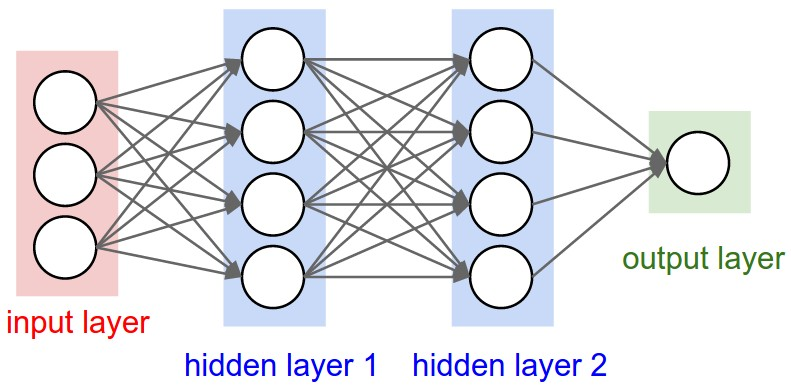
\includegraphics[width=0.7\linewidth]{neural_net2.jpeg}}
  \caption{An example of a 2-layer neural network~\cite{Kar16}.}
  \label{fig:neural-network}
\end{figure}

There are numerous neural network classifications depending on their architecture; the design relevant to this thesis is \textit{supervised}\footnote{As in ``supervised learning", a concept in machine learning where a set of training examples is paired up with a set of corresponding desired output values. A supervised neural network thus adjusts its links' weights to get the correct output values during its training phase.} FFBP neural network. Its training process and mathematical representation are briefly outlined in \ref{sec:training}.

Finally,~\cite{Nor14} summarises the attractiveness of neural networks as follows: (1) its capacity to support parallel computation; (2) its fault tolerant nature against novel inputs; (3) \textit{Graceful degradation}, which means a gradual performance drop-offs in worsening conditions; and, (4) The usage of inductive learning algorithms to train the networks.

\section{Feed-forward back-propagation learning algorithm}\label{sec:training}

This section explains the mechanics and the mathematical representation involved in training a fully-connected, supervised FFBP neural network, based on the works in~\cite{Ng12}. Given a set of features and training samples, this learning algorithm aims to find the correct weight distribution in the neural network in two stages: \textit{feed-forward propagation} and \textit{back-propagation}. 

First, the weights are randomly initialised within the permitted range of the chosen activation function. For example, this range is $[0,1]$ for a sigmoid function; for a tanh function, it is $[-1,1]$. 

Now, in a $k$-layer neural network, let the size or the number of units in layer $j$ be denoted as $|j|$. Let a particular training sample, $s$, be denoted as $(\boldsymbol{x}^{(s)},\boldsymbol{y}^{(s)})$, such that $\boldsymbol{x}^{(s)} = [x_1^{(s)},...,x_m^{(s)}]$ is the sample input and $\boldsymbol{y}^{(s)} = [y_1^{(s)},...,y_n^{(s)}]$ is the matching desired output. Let $a_{i}^{(j)}$ be the activation value of unit $i$ in layer $j$, where $1 \leq i \leq |j|$, $1 \leq j \leq k$. Let $g(x)$ be the activation function; $\Theta_{qp}^{(j)}$ be the weight of a link from unit $p$ in layer $j$ to unit $q$ in layer $j+1$; and, let $\Theta^{(j)}=[\Theta{qp}^{(j)} \text{ for } 1\leq q \leq |j+1|, 1 \leq p \leq |j|]$ be the matrix of weights controlling function mapping from layer $j$ to $j+1$.

Then we can express $a_{i}^{(j)}$ as,
\begin{equation}
a_{i}^{(j)} = g( \Theta_{i1}^{(j-1)}a_{1}^{(j-1)} + \Theta_{i2}^{(j-1)}a_{2}^{(j-1)} + ...+\Theta_{i|j-1|}^{(j-1)}a_{|j-1|}^{(j-1)} ) \label{eq:2.1}
\end{equation}
For instance, the activation of unit $i$ in the first hidden layer can be expressed as,
$$a_{i}^{(2)} = g(\Theta_{i1}^{(1)}x_{1}^{(s)} + ... + \Theta_{im}^{(1)}x_{m}^{(s)})$$
and, in the output layer as~\cite{Ng12},
$$a_{i}^{(k)} = g(\Theta_{i1}^{(k-1)}a_{1}^{(k-1)} + ...+\Theta_{i|k-1|}^{(k-1)}a_{|k-1|}^{(k-1)})$$ 
Also, unlike the approach taken above by Ng (2016),~\cite{Kar16} states that the activation function is not commonly applied to output layer, because often the result as a real-value number received by the outer layer is the information sought by the user.

\ref{eq:2.1} can be simplified using vectorised implementation. Let the activated units in layer $j$ be denoted as $a^{(j)} = [a_{1}^{(j)},...,a_{|j|}^{(j)}]$. Then inputs to this layer can be expressed as $z^{(j)} = \Theta^{(j-1)} a^{(j-1)}$ and so $a^{(j)}$ becomes,
\begin{equation}
a^{(j)} = g(z^{(j)}) \label{eq:2.2}
\end{equation}
Forward-propagation process ends when the input values are thus propagated to the output layer. 

Next, back-propagation involves re-distributing the error value between the expected output, $\boldsymbol{y}^{(s)}$, and actual output, $a^{(k)}$, back from the output layer through the hidden layers~\cite{RumHinWil86}. This concept is based on the idea that the previous layer is responsible for some fraction of the error in next layer, proportional to the links' weights. 

Let $\delta_i^{(j)}$ denote the error value in unit $i$ in layer $j$ and $\delta^{(j)} = [\delta_1^{(j)},...,\delta_{|j|}^{(j)}]$ be the vectorised error values. Then, for $1 < j < k$,
\begin{equation}
\delta^{(j)} = (\Theta^{(j)})^{T} \delta^{(j+1)} .\!* g'(z^{(j)})
\end{equation}
where $.\!*$ is an element-wise multiplication. The error in the output layer is $\delta^{(k)} = a^{(k)} - \boldsymbol{y}^{(s)}$ and that there is no error in the first layer, because as input values, they cannot contain error.

Finally, the error in link weight $\Theta_{qp}^{(j)}$ is denoted as $\Delta_{qp}^{(j)}$, such that,
$$\Delta_{qp}^{(j)}  = a_p^{(j)}\delta_q^{(j+1)}$$
This, too, can be simplified using vectorised implementation as,
\begin{equation}
\Delta^{(j)} = \delta^{(j+1)}(a^{(j)})^T \label{eq:2.3}
\end{equation}
Back-propagation ends for $s$ when the errors from the output layer is propagated to the first hidden layer.

The FFBP learning algorithm is then repeated for all the training samples. $\Delta^{(j)}$ accumulates all the errors in the training set during this process. Once the process is finished, the final values are averaged out by the size of the training set, a \textit{regularisation term} is added, and finally the weights are updated. A regularisation term is a value that is added in gradient descent algorithm in machine learning, to prohibit features that are vastly different in its range of input values from one another from distorting the results~\cite{Ng12}. This entire process is also known as a form of \textit{batch gradient descent} (BGD) learning algorithm in machine learning~\cite{Ng12} and is the method chosen to implement my Accelerate neural network (see Chapter~\ref{ch:impl}.

There are other advanced optimization methods that can improve the performance of neural networks, but these have yet to be explored at the time of this report. As with other machine learning algorithms, the performance may also be improved with either altering various parameters, such as regularisation parameter $\lambda$ and the learning rate parameter $\alpha$, altering the number of features, gaining more training examples, adding polynomial features, or any combination of these~\cite{Ng12}. However, \textit{diagnostic analysis} is often the fastest and most economically sound method to determine which set of features is effective~\cite{Ng12}. Diagnostic analysis is a form of trial-and-error testing of features sets, or \textit{hypotheses}, with a small set of training examples to assess its performance and thus its suitability.

\section{GPU-accelerated programming and neural networks}\label{se:gpu}

Neural networks implemented with GPU-accelerated programming have shown a significant performance improvement. For instance,~\cite{OhJun04} had a 20-fold performance enhancement of a multi-layered perceptron (MLP) network to detect text using an ATI RADEON 9700 PRO in 2004. More recently,~\cite{GurFor13} showed that performance gains from parallel implementation of neural networks in GPUs are scalable with the processing power of the GPU used. Their results show that performance enhancement over the pure CPU implementation increased with data set size before reaching a plateau, a limit which they contribute to the saturation of the GPU's processing cores.

~\cite{Nvi14} explains that GPU computing is particularly well-suited to neural networks due to its massively parallel architecture, consisting of tens of thousands of cores. Thus, as single GPUs can hold entire neural network, they state that neural networks benefit from an overall bandwidth increase, reduction in communication latency, and a decrease in size and power consumption compared to a CPU cluster. Furthermore, as neural network units essentially repeat the same computation only with differing input values, the algorithm complements the GPU architecture as there is minimal need for conditional instructions that could trigger thread divergences, which can dramatically reduce the GPU throughput.

The main GPU programming language is CUDA, an API model created by NVIDIA in 2007. It has a C/C++ language style and the added benefits that it bypasses the need to learn graphics shading languages or learn about computer graphics in order to program the GPU. The alternative to CUDA is Open Computing Language (OpenCL) released in 2009; also based on C/C++, it is considered to be the more complicated language of the two, but with enhanced portability. As both languages are very low-level~\cite{Mar13}, there is a need for a way to create, manipulate and test neural networks in less complicated, more user-friendly, safer, higher-level language, such as a functional language.

\section{Accelerate}\label{se:accelerate}

Accelerate is an Embedded Domain-Specific Language (EDSL) for GPU programming, released by UNSW PLS in 2011. EDSLs are restricted languages that are embedded in a more powerful language, so as to reuse the host language's infrastructure and enable powerful metaprogramming. In the case of Accelerate, Haskell is the host language and it compiles into CUDA code that runs directly on the GPU. 

\begin{figure}
  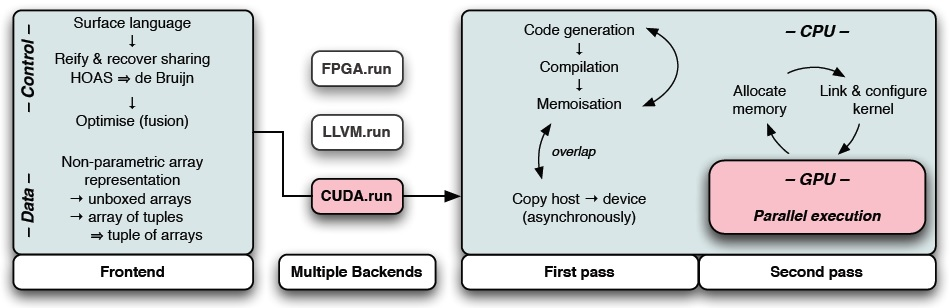
\includegraphics[width=\linewidth]{accelerate-structure.jpg}
  \caption{Structure overview of \texttt{Data.Array.Accelerate}.~\cite{ChaKelLee11}}
  \label{fig:acc-struct}
\end{figure}

Accelerate provides a framework for programming with arrays~\cite{Mar13} -- Accelerate programs take arrays as input and output one or more arrays. The type of Accelerate arrays is,
$$\texttt{data Array sh e}$$
where \texttt{sh} is the \textit{shape}, or dimensionality of the array, and \texttt{e} is the \textit{element type}, for instance \texttt{Double}, \texttt{Int} or tuples. However, \texttt{e} cannot be an array type; that is, Accelerate does not support nested arrays. This is because GPUs only have flat arrays and do not support such structures~\cite{Mar13}. 

Types of array shapes and indices are shown in Fig. \ref{fig:acc-types}~\cite{ChaKelLee11}. It shows that the simplest shape is \texttt{Z}, which is the shape of an array with no dimensions and a single element, or a scalar. A vector is represented as \texttt{Z:.Int}, which is the shape of an array with a single dimension indexed by \texttt{Int}. Likewise, the shape of a two-dimensional array, or matrix, is \texttt{Z:.Int:.Int} where the left and right \texttt{Int}s denotes the row and column indexes or numbers, respectively.

\begin{figure}
  \centerline{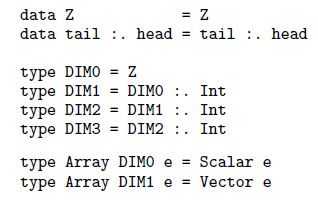
\includegraphics[width=0.5\linewidth]{accelerate-types.jpg}}
  \caption{Types of array shapes and indices~\cite{ChaKelLee11}.}
  \label{fig:acc-types}
\end{figure}

Common shapes have type synonyms, such as scalars as \texttt{DIM0}, vectors as \texttt{DIM1} and matrices as \texttt{DIM2}. Similarly, common array dimensions of zero and one also have type synonyms as \texttt{Scalar e}, \texttt{Vector e}, respectively.

Arrays can be built using \texttt{fromList}; for instance, a $2 \times 5$ matrix with elements numbered from 1 to 10 can be created with,
$$\texttt{fromList (Z:.2:.5) [1..]::Array DIM2 Int}$$

To do an actual Accelerate computation on the GPU, there are two options~\cite{Mar13}:
\begin{enumerate}
\item Create arrays within the Haskell world. Then, using \texttt{use}, inject the array \texttt{Array a} into the Accelerate world as \texttt{Acc (Array a)}. Then, use \texttt{run}.
\item Create arrays within the Accelerate world. There are various methods, such as using \texttt{generate} and \texttt{fill}. Then, use \texttt{run}.
\end{enumerate}
\texttt{run} executes the Accelerate computation and copies the final values back into Haskell after execution. In \texttt{Acc a}, \texttt{Acc} is an Accelerate data structure representing a computation in the Accelerate world, that yields a value of type \texttt{a} (more specifically, an array) \textit{once it is executed by a backend}~\cite{McD13, Mar13}. 

Now, as the first method may require the array data to be copied from computer's main memory into the GPU's memory, the second method is generally more efficient~\cite{Mar13}. All the aforementioned functions are outlined in Fig. \ref{fig:acc-functions}.
\begin{figure}
  \begin{lstlisting}
    -- build an array in Haskell world
    fromList :: (Shape sh, Elt e) => sh -> [e] -> Array sh e

	-- to execute an Accelerate computation on the GPU
    run :: Arrays a => Acc a -> a
    
    -- inject Haskell world array into Accelerate world
    use :: Arrays arrays => arrays -> Acc arrays
    
    -- create an array in Accelerate world (array filled with user-specified function)
    generate :: (Shape ix, Elt a) 
              => Exp ix -> (Exp ix -> Exp a) -> Acc (Array ix a)
    
    -- create an array in Accelerate world (array filled with same values)
    fill :: (shape sh, Elt e) => Exp sh -> Exp e -> Acc (Array sh e)
  \end{lstlisting}
  \caption{Some Accelerate functions~\cite{Mar13}.}
  \label{fig:acc-functions}
\end{figure}

Since Accelerate has its own backend compiler, it must be set before any code can be \texttt{run}. There can be a number of backends to execute Accelerate computations: (1) \texttt{Data.Array.Accelerate.Intepreter}, the slowest performing, simple Haskell interpreter; (2) \texttt{accelerate-llvm-native}, which supports parallel execution on multicore CPUs; and, (3) \texttt{accelerate-llvm-ptx}, which supports parallel execution on CUDA-capable NVIDIA GPUs. \texttt{accelerate-cuda} is deprecated in favour of (3).

Further details about the Accelerate language is continued in \ref{se:previmplem}.

\section{Previous Implementations in Accelerate} \label{se:previmplem}

A neural network in Accelerate is a fairly new concept and as such, there is only one known work in~\cite{Eve16}. In it, Everest (2016) implements a FFBP neural network with a \textit{stochastic gradient descent} (SGD) learning algorithm, based on a Python implementation~\cite{Nie16}. This section briefly covers the details of this implementation.

SGD algorithm is a modification of BGD algorithm, shown in \ref{sec:training}. Rather than adjusting the neural network parameters after going through the entire training set, SGD updates the parameters immediately after doing the FFBP algorithm for a single training example, which is picked at random~\cite{Ng12}. SGD can also be modified to select certain small batches of training sample at a time~\cite{LeC98}. 

As such, SGD is computationally less expensive than the BGD, and allows the training algorithms to scale better to much larger training sets~\cite{Ng12}. ~\cite{LeCBosDen89} also claims that SGD trains the neural network faster. The disadvantages of SGD are that it is said to be "less accurate" than BGD as it may take longer to reach the local/global minima, however, it is still the more popular choice due to less strain it puts on the system. Also, SGD is suitable to the work in~\cite{Eve16}, because it deals with processing data streaming.

There are six key Accelerate functions that were used and their names and operations are listed in Fig. \ref{fig:acc-functions2}. These functions were also used in my own implementation (see Chapter\~ref{ch:impl}). In particular, the functions \texttt{lift} and \texttt{unlift} are used to inject and extract a value into and out of \texttt{Exp}\footnote{\texttt{Exp} is another Accelerate data structure, that is similar to \texttt{Acc} (refer to \ref{se:accelerate}), but instead of an array, it represents an embedded \textit{scalar} computation~\cite{ChaKelLee11}.}, respectively, and are thus essential in interpreting the indices of arrays in Accelerate~\cite{Mar13}.

\begin{figure}
  \begin{lstlisting}
    -- apply supplied function element-wise to corresponding elements of two input arrays to produce a third array 
    zipWith :: (Shape ix, Elt a, Elt b, Elt c)
             => (Exp a -> Exp b -> Exp c)
             -> Acc (Array ix a) -> Acc (Array ix b) -> Acc (Array ix c)

	-- map function within the Accelerate world
    map :: (Shape ix, Elt a, Elt b)
         => (Exp a -> Exp b) -> Acc (Array ix a) -> Acc (Array ix b)
    
    -- replicate an array across one or more dimensions according to the first argument (a generalised array index)
    replicate :: (Slice slix, Elt e)
               => Exp slix -> Acc (Array (SliceShape slix) e)
               -> Acc (Array (FullShape slix) e)
    
    -- reduce the innermost dimension of an array
    fold :: (Shape ix, Elt a)
          => (Exp a -> Exp a -> Exp a) -> Exp a
          -> Acc (Array (ix:.Int) a) -> Acc (Array ix a)
          
    -- wraps a value in Exp
    lift :: Z:.Exp Int:.Exp Int -> Exp (Z:.Int:.Int)
    
    -- deconstruct Exp, get the structured value from within
    unlift :: Exp (Z:.Int:.Int) -> Z:.Exp Int:.Exp Int
  \end{lstlisting}
  \caption{Key Accelerate functions used in~\cite{Eve16}.}
  \label{fig:acc-functions2}
\end{figure}

In~\cite{Eve16}, two support functions were also created to assist forward- and back-propagation processes -- \texttt{mvm} and \texttt{cross} (see Fig. \ref{fig:acc-functions3}).
\begin{figure}
\begin{lstlisting}
  -- matrix vector multiplication function
  mvm :: (Elt a, IsNum a)
       => Acc (Matrix a) -> Acc (Vector a) -> Acc (Vector a)
  mvm mat vec
    = let Z:.h:._ = unlift (shape mat) :: Z:.Exp Int:.Exp Int
    in A.fold (+) 0 $ A.zipWith (*) mat (A.replicate (A.lift (Z:.h:.All)) vec)
  
  -- vector multiplication function
  cross :: Acc (Vector Float) -> Acc (Vector Float) -> Acc (Matrix Float)
  cross v h = A.zipWith (*) (A.replicate (lift (Z:.All:.size h)) v)
                               (A.replicate (lift (Z:.size v:.All)) h)
\end{lstlisting}
  \caption{Support functions for forward- and back-propagation used in~\cite{Eve16}.}
  \label{fig:acc-functions3}
\end{figure}
In \texttt{mvm}, \texttt{h} first stores the row number of the matrix input using \texttt{unlift}. The vector input, \texttt{vec} is then replicated \texttt{h} times across the first dimension using \texttt{replicate}. The resulting matrix is then element-wise multiplied with \texttt{mat} using \texttt{zipWith}. Lastly, the values of the matrix are summed and flattened back into a vector using \texttt{fold}.

The process is similar in \texttt{cross}. \texttt{cross} is a vector multiplication function that returns a matrix. First, vector \texttt{v} is replicated $|h|$ number of times in the second dimension, whereas vector \texttt{h} is replicated $|v|$ number of times in the first dimension. The resulting two matrices are then element-wise multiplied using \texttt{zipWith}. 

The actual FFBP algorithm is in the function \texttt{backprop}. In \texttt{backprop}, Accelerate code (imported as \texttt{A}) seamlessly interweaves with the Haskell part (imported as \texttt{P}), as seen in Fig. \ref{fig:acc-functions4}.
\begin{figure}
  \begin{lstlisting}
  -- back-propagation part of backprop function
  nabla_b_final = A.zipWith (*) ( costDerivative (P.last activations) y) 
                                                 (A.map sigmoid' (P.last zs) )
  nabla_w_final = cross nabla_b_final ( P.last (P.init activations) )
  
  ...
  \end{lstlisting}
  \caption{Accelerate and Haskell code are mixed in~\cite{Eve16}.}
  \label{fig:acc-functions4}
\end{figure}

At the time of this report, ~\cite{Eve16} has reported some performance issues with this implementation with the success rate of digit prediction at appropriximately 50\%. The cause is yet unknown, but may possibly be due to the nature of data streaming. This implementation also purportedly running at a slower speed than an equivalent Theano implementation. Theano is a Python library that is optimised for multi-dimensional array computations, and can be optimised to use GPU for computations.